\documentclass[a4paper,10pt]{article}
\title{}
\author{}
\usepackage{graphicx} 

\begin{document}
\maketitle
\begin{abstract}

We consider the single parametered family of triangles in the hyperbolic two dimensional space that have two angles of size zero and one non zero angle.
More specifically we are interested in the Fangano triangles formed by connecting the bases of the (hyperbolic) heights of the triangles as shown in Figure 1, modeled as will be the whole document 
in the upper half plane model:

\begin{center}
 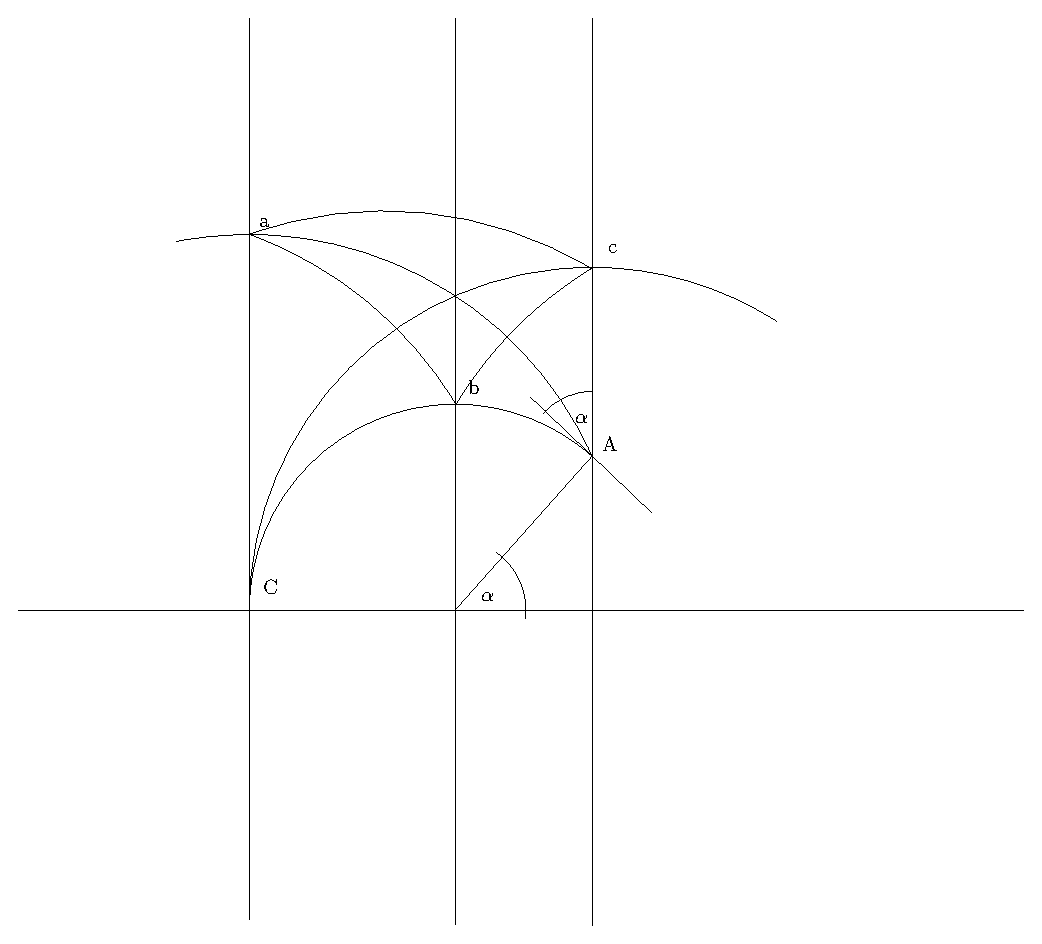
\includegraphics[width=12cm]{./hyper00a.eps}
 % hyper00a.eps: 0x0 pixel, 300dpi, 0.00x0.00 cm, bb=41 259 525 696
 Figure 1
\end{center}

Our goal is to understand what $\alpha$ maximizes the perimiter of such triangles.
We will see that the perimiter of such inner triangles as a function of the free
angle will of the outer triangle has only one critial point within
the interval $\left[0,\frac{pi}{2}\right)$ located at zero and is thus monotoneus
and can easily shown to be decreasing. We will conclude the maximal perimiter of
the Fangano triangle is given in the equilateral triangle with angles 0-0-0.

\end{abstract}
\section{}

Let us first find $A'$, $B'$ and $C'$, the bases of the heights.

Since $B$ is located at $\infty$, it is trivial to see that

\begin{center}
$B' = 1 + i$ 
\end{center}

Since it is the only perpendicular to the euclidean circle that represents the
edge $AC$ that originates in $\infty$ of the $H^2$ model.

Now, since the edges leaving $A$ and $C$ towards $B$ (located at $\infty$) are
perpendicular to the real axis, every hyperbolic line perpendicular to them
is positioned along Euclidean circle centered at the edge's meeting with the
real axis.

Knowing the above, it is easy to calculate the point the perpendiculars cross
the opposie edges, the center we have shown is the edge's meeting point with the
real axis and the radius is the Euclidean distance between the veterx and the 
opposite edge:

\begin{center}
$A' = i \sqrt{2 + 2 cos\left(\alpha\right)}$


$C' = \left(1 + i\right) \left(1 + cos\left(\alpha\right)\right)$
\end{center}


Now let us calculate the hyperbolic distances between $a$, $b$ and $c$ using the formula:

\begin{center}

$d\left(x,y\right) = acosh(\frac{\|x-y\|^{2}}{\Im\left(x\right)\Im\left(y\right)})$


\end{center}

\noindent$d\left(A', B'\right) =$

$acosh\left(1 + \frac{\left(\Im\left(A' - B'\right)\right)^{2} + \left(\Re\left(A' - B'\right)\right)^{2}}{2 \sqrt{2 + 2 cos\left(\alpha\right)}}\right) =$
$acosh\left(1 + \frac{1 + \left(1 - \sqrt{2 + 2 cos\left(\alpha\right)}\right)^{2}}{2 \sqrt{2 + 2 cos\left(\alpha\right)}}\right) =$

$acosh\left(1 + \frac{4 + 2 cos\left(\alpha\right) - 2 \sqrt{2 + 2 cos\left(\alpha\right)}}{2 \sqrt{2 + 2 cos\left(\alpha\right)}}\right) =$
$acosh\left(\frac{4 + 2 cos\left(\alpha\right)}{2 \sqrt{2 + 2 cos\left(\alpha\right)}}\right) =$

$acosh\left(\frac{2 + cos\left(\alpha\right)}{\sqrt{2 + 2 cos\left(\alpha\right)}}\right) $



\noindent$d\left(B', C'\right) = $

$acosh\left(1 + \frac{\left(\Im\left(B' - B'\right)\right)^{2} + \left(\Re\left(B' - C'\right)\right)^{2}}{2 + 2 cos\left(\alpha\right)}\right) =$
$acosh\left(1 + 2 \frac{cos^{2}\left(\alpha\right)}{2 + 2 cos\left(\alpha\right)}\right) =$

$acosh\left(1 + \frac{cos^{2}\left(\alpha\right)}{1 + cos\left(\alpha\right)}\right) =$
$acosh\left(\frac{1 + cos\left(\alpha\right) + cos^{2}\left(\alpha\right)}{1 + cos\left(\alpha\right)}\right) $


\noindent$ d\left(C', A'\right)=$

$acosh\left(1 + \frac{\left(\Im\left(C' - A'\right)\right)^{2} + \left(\Re\left(C' - A'\right)\right)^{2}}{\left(2 + 2 cos\left(\alpha\right)\right)^{\frac{3}{2}}}\right) =$
$acosh\left(1 + \frac{\left(1 + cos\left(\alpha\right)\right)^{2} + \left(1 + cos\left(\alpha\right) - \sqrt{2 + 2 cos\left(\alpha\right)}\right)^{2}}{\left(2 + 2 cos\left(\alpha\right)\right)^{\frac{3}{2}}}\right) =$

$acosh\left(1 + \frac{3 + 4 cos\left(\alpha\right) + \left(1 + cos\left(\alpha\right)\right)^{2} + cos^{2}\left(\alpha\right) - \left(2 + 2 cos\left(\alpha\right)\right)^{\frac{3}{2}}}{\left(2 + 2 cos\left(\alpha\right)\right)^{\frac{3}{2}}}\right) =$
$acosh\left(1 + \frac{4 + 6 cos\left(\alpha\right) + 2 cos^{2}\left(\alpha\right) - \left(2 + 2 cos\left(\alpha\right)\right)^{1.5}}{\left(2 + 2 cos\left(\alpha\right)\right)^{\frac{3}{2}}}\right) =$

$acosh\left(1 + \frac{4 + 6 cos\left(\alpha\right) + 2 cos^{2}\left(\alpha\right) - \left(2 + 2 cos\left(\alpha\right)\right)^{1.5}}{\left(2 + 2 cos\left(\alpha\right)\right)^{\frac{3}{2}}}\right) =$
$acosh\left(1 + \frac{4 + 6 cos\left(\alpha\right) + 2 cos^{2}\left(\alpha\right) - \left(2 + 2 cos\left(\alpha\right)\right)^{1.5}}{\left(2 + 2 cos\left(\alpha\right)\right)^{1.5}}\right) =$

$acosh\left(\frac{4 + 6 cos\left(\alpha\right) + 2 cos^{2}\left(\alpha\right)}{\left(2 + 2 cos\left(\alpha\right)\right)^{1.5}}\right) =$
$acosh\left(\frac{\sqrt{2} \left(2 + 3 cos\left(\alpha\right) + cos^{2}\left(\alpha\right)\right)}{\left(1 + cos\left(\alpha\right)\right)^{1.5}}\right) =$

$acosh\left(\frac{\sqrt{2} \left(2 + 3 cos\left(\alpha\right) + cos^{2}\left(\alpha\right)\right)}{2 \left(1 + cos\left(\alpha\right)\right)^{1.5}}\right) =$
$acosh\left(\frac{2 + cos\left(\alpha\right)}{\sqrt{2 + 2 cos\left(\alpha\right)}}\right)$

\noindent
We notice that
\begin {center}
$ d\left(a, c\right)=d\left(a, b\right) $
\end {center}



\noindent
We differentiate each distance expression (with respect to $\alpha$):




\noindent$\frac{d}{d\alpha}d\left(A', B'\right)=\frac{d}{d\alpha}d\left(C', A'\right)=$

$\frac{- \frac{sin\left(\alpha\right)}{\left(2 + 2 cos\left(\alpha\right)\right)^{0.5}} + 2 \frac{\left(1.0 + 0.5 cos\left(\alpha\right)\right) sin\left(\alpha\right)}{\left(2 + 2 cos\left(\alpha\right)\right)^{1.5}}}{\left(-1 + \frac{\left(2 + cos\left(\alpha\right)\right)^{2}}{2 + 2 cos\left(\alpha\right)}\right)^{0.5}}=$
$\sqrt{\frac{2 + 2 cos\left(\alpha\right)}{2 + 2 cos\left(\alpha\right) + cos^{2}\left(\alpha\right)}} \left(- \frac{sin\left(\alpha\right)}{\left(2 + 2 cos\left(\alpha\right)\right)^{0.5}} + 2 \frac{\left(1.0 + 0.5 cos\left(\alpha\right)\right) sin\left(\alpha\right)}{\left(2 + 2 cos\left(\alpha\right)\right)^{1.5}}\right)=$

$- \frac{\sqrt{\frac{2 + 2 cos\left(\alpha\right)}{2 + 2 cos\left(\alpha\right) + cos^{2}\left(\alpha\right)}} \left(1 - \frac{2 + cos\left(\alpha\right)}{2 + 2 cos\left(\alpha\right)}\right) sin\left(\alpha\right)}{\sqrt{2 + 2 cos\left(\alpha\right)}}=$
$- \frac{\sqrt{\frac{2 + 2 cos\left(\alpha\right)}{2 + 2 cos\left(\alpha\right) + cos^{2}\left(\alpha\right)}} cos\left(\alpha\right) sin\left(\alpha\right)}{\left(2 + 2 cos\left(\alpha\right)\right)^{\frac{3}{2}}}=$

$- \sqrt{\frac{1}{\left(2 + 2 cos\left(\alpha\right)\right)^{2} \left(2 + 2 cos\left(\alpha\right) + cos^{2}\left(\alpha\right)\right)}} cos\left(\alpha\right) sin\left(\alpha\right)=$
$- \frac{cos\left(\alpha\right) sin\left(\alpha\right)}{\sqrt{2 + 2 cos\left(\alpha\right) + cos^{2}\left(\alpha\right)} \left(2 + 2 cos\left(\alpha\right)\right)}$


\noindent$\frac{d}{d\alpha}d\left(B',C'\right)=$

$\frac{cos^{2}\left(\alpha\right) sin\left(\alpha\right) - 2 \left(1 + cos\left(\alpha\right)\right) cos\left(\alpha\right) sin\left(\alpha\right)}{\left(1 + cos\left(\alpha\right)\right)^{2} \left(-1 + \frac{\left(1 + cos\left(\alpha\right) + cos^{2}\left(\alpha\right)\right)^{2}}{\left(1 + cos\left(\alpha\right)\right)^{2}}\right)^{0.5}}=$
$\frac{cos^{2}\left(\alpha\right) sin\left(\alpha\right) - 2 \left(1 + cos\left(\alpha\right)\right) cos\left(\alpha\right) sin\left(\alpha\right)}{\left(1 + cos\left(\alpha\right)\right)^{2} \left(-1 + \left(1 + \frac{cos^{2}\left(\alpha\right)}{1 + cos\left(\alpha\right)}\right)^{2}\right)^{0.5}}=$

$\frac{cos^{2}\left(\alpha\right) sin\left(\alpha\right) - 2 \left(1 + cos\left(\alpha\right)\right) cos\left(\alpha\right) sin\left(\alpha\right)}{\left(1 + cos\left(\alpha\right)\right)^{2} \left(2 \frac{cos^{2}\left(\alpha\right)}{1 + cos\left(\alpha\right)} + \frac{cos^{4}\left(\alpha\right)}{\left(1 + cos\left(\alpha\right)\right)^{2}}\right)^{0.5}}=$
$\frac{cos^{2}\left(\alpha\right) sin\left(\alpha\right) - 2 \left(1 + cos\left(\alpha\right)\right) cos\left(\alpha\right) sin\left(\alpha\right)}{\left(\frac{2 + 2 cos\left(\alpha\right) + cos^{2}\left(\alpha\right)}{\left(1 + cos\left(\alpha\right)\right)^{2}}\right)^{0.5} \left(1 + cos\left(\alpha\right)\right)^{2} cos\left(\alpha\right)}=$

$\frac{cos^{2}\left(\alpha\right) sin\left(\alpha\right) - 2 \left(1 + cos\left(\alpha\right)\right) cos\left(\alpha\right) sin\left(\alpha\right)}{\sqrt{2 + 2 cos\left(\alpha\right) + cos^{2}\left(\alpha\right)} \left(1 + cos\left(\alpha\right)\right) cos\left(\alpha\right)}=$
$\frac{cos^{2}\left(\alpha\right) sin\left(\alpha\right) - 2 \left(1 + cos\left(\alpha\right)\right) cos\left(\alpha\right) sin\left(\alpha\right)}{\sqrt{2 + 2 cos\left(\alpha\right) + cos^{2}\left(\alpha\right)} \left(1 + cos\left(\alpha\right)\right) cos\left(\alpha\right)}=$

$\frac{\left(- \left(2 + 2 cos\left(\alpha\right)\right) cos\left(\alpha\right) + cos^{2}\left(\alpha\right)\right) sin\left(\alpha\right)}{\sqrt{2 + 2 cos\left(\alpha\right) + cos^{2}\left(\alpha\right)} \left(1 + cos\left(\alpha\right)\right) cos\left(\alpha\right)}=$
$- \frac{\left(2 + cos\left(\alpha\right)\right) sin\left(\alpha\right)}{\sqrt{2 + 2 cos\left(\alpha\right) + cos^{2}\left(\alpha\right)} \left(1 + cos\left(\alpha\right)\right)}$

\noindent
And sum the three up:

\noindent$\frac{d}{d\alpha}\left(d\left(A', B'\right) + d\left(B', C'\right) + d\left(C', A'\right)\right) = $

$\frac{d}{d\alpha}\left(2d\left(A', B'\right) + d\left(B', C'\right)\right) = $

$2\frac{d}{d\alpha}d\left(A', B'\right) + \frac{d}{d\alpha}d\left(B', C'\right) = 
 - \frac{\left(2 + cos\left(\alpha\right)\right) sin\left(\alpha\right)}
        {\sqrt{2 + 2 cos\left(\alpha\right) + cos^{2}\left(\alpha\right)} \left(1 + cos\left(\alpha\right)\right)} - $

  
$  2\frac{cos\left(\alpha\right) sin\left(\alpha\right)}
  {\sqrt{2 + 2 cos\left(\alpha\right) + cos^{2}\left(\alpha\right)} \left(2 + 2 cos\left(\alpha\right)\right)} =$

$  \frac{-\left(2 + cos\left(\alpha\right)\right) sin\left(\alpha\right) - cos\left(\alpha\right) sin\left(\alpha\right)}{\sqrt{2 + 2 cos\left(\alpha\right) + cos^{2}\left(\alpha\right)} \left(1 + cos\left(\alpha\right)\right)} $

$- \frac{2sin\left(\alpha\right)\left(1 + cos\left(\alpha\right)\right)}{\sqrt{2 + 2 cos\left(\alpha\right) + cos^{2}\left(\alpha\right)\left(1 + cos\left(\alpha\right)\right)}} =$
$- \frac{2sin\left(\alpha\right)}{\sqrt{2 + 2 cos\left(\alpha\right) + cos^{2}\left(\alpha\right)}}$

\noindent
We end up with an expression that is negative and null only at zero (within the
interval $\left[0,frac{\pi}{2}\right)$) and can conclude that the maximal perimiter
of the Fangano triangle is achieved at $\alpha = 0$. Its perimiter is:

\begin{center}
$2acosh\left(\frac{2 + cos\left(0\right)}{\sqrt{2 + 2 cos\left(0\right)}}\right) + 
acosh\left(\frac{1 + cos\left(0\right) + cos^{2}\left(0\right)}{1 + cos\left(0\right)}\right) =
3acosh\left(\frac{3}{2}\right)$
\end{center}


Appendix: proof the triangle connecting the bases of the heights of such triangles 
is indeed the Fangano orbit

We will achieve the above by finding the equations of the edges and showing the
angles of intersection with the edges are equal to each other, which is easy to
see means the deriviative's are equal in absolute values but opposite in sign.


First we calculate the centers of the Euclidean circles along which the edges
of the inner triangle $A'B'C'$ lay using the formula:

\begin{center}
  $c\left(x,y\right) = \frac{\left|x\right|**2 - \left|x\right|**2}{2\left(\Re(x) - \Re(y)\right)} $
\end{center}

Where $c\left(x,y\right)$ represents the center of the Euclidean circle passing
through $x$ and $y$.

  $c\left(A',B'\right) = \left(2 + 2\cos\left(\alpha\right) - 2\right) / {2\left(0 - 1\right)} = -cos(\alpha) $

  $c\left(A',B'\right) = \left(2 - 2*\left(1+ cos\left(\alpha\right)\right)**2\right) / \left(2*\left(1 - 1 -  cos\left(a\right)\right)\right), 
    cos\left(\alpha\right) + 2 = cos\left(\alpha\right)$

  $c\left(C',A'\right) = \frac{2\left(1 + cos\left( \alpha \right) \right)^2 - \left(2 + 2cos\left(\alpha\right)\right)} 
                                         {2\left(1+cos\left(\alpha \right) \right)}    $


It is easy to show hat the differential equation describing a circle whose center
$r$ is on the real axis can be written as:

$2\left(x-r\right)+2yy'=0$

Sustitutibg the above calculated centers:
  
\noindent $AB$ :  $y' = -\frac{x + cos\left(\alpha \right)}{ y} $

\noindent $BC$ :  $y' = -\frac{x - cos\left(a\right) - 2}{y}$

\noindent $CA$ :  $y' = -\frac{x - cos\left(a\right)}{y}$


Substituting $(x,y)$ for the real and imaginary parts of the endpoints $A'$,$B'$,$C'$ we get:

\noindent $A$: 

on $CA$ : $-\frac{-cos\left(\alpha \right)}{\sqrt{2 + 2 cos\left(\alpha\right)}}$

on $AB$ : $-\frac{cos\left(\alpha \right)}{\sqrt{2 + 2 cos\left(\alpha\right)}}$

\noindent $B$: 
on $AB$ : $-\left(1 + cos\left(\alpha \right)\right)$

on $BC$ : $-\left(1 - cos\left(\alpha \right) - 2\right)$ =  $1 + cos\left(\alpha \right)$

\noindent $C$: 

on $BC$ : $-\frac{1 + cos\left(\alpha\right) - cos\left(a\right) - 2}{1 + cos\left(\alpha\right)} = \frac{1}{1 + cos\left(\alpha\right)}$

on $CA$ : $-\frac{1 + cos\left(\alpha\right) - cos\left(a\right)    }{1 + cos\left(\alpha\right)} = -\frac{1}{1 + cos\left(\alpha\right)}$

\end{document}


$B' = 1 + i$ 

$A' = i \sqrt{2 + 2 cos\left(\alpha\right)}$


$C' = \left(1 + i\right) \left(1 + cos\left(\alpha\right)\right)$

